% ============================================================
% MX MODEL  — slides (texto original preservado; incorporados:
%   (1) figura de IRFs do MX (fig_mx_ir.png),
%   (2) Tabela 7.6 (table_7_6.txt),
%   (3) Tabela 7.7 por país (table_7_7_bycountry.csv).
% Compilar: pdflatex mx_model_slides.tex  (fig_mx_ir.png na mesma pasta)
% ============================================================
\documentclass[10pt]{beamer}
\usetheme{Madrid}
\usecolortheme{seahorse}
\usepackage{amsmath}
\usepackage{booktabs}
\usepackage{graphicx}
\beamertemplatenavigationsymbolsempty

\title{The MX Model}
\subtitle{Importable Goods, Exportable Goods, and the Terms of Trade}
\date{}

\begin{document}

\begin{frame}\titlepage\end{frame}

% ------------------------------------------------------------
% 1. MOTIVATION
% ------------------------------------------------------------
\begin{frame}{The MX Model: Why Do We Need It?}
\small
\begin{itemize}
    \item So far, the empirical SVAR has shown how the economy
    \textbf{responds to Terms-of-Trade shocks}.
    \item But the previous one-good framework treats the ToT shock
    essentially as a productivity shock.
    \item This implies an unrealistic economy in which:
    \begin{itemize}
        \item virtually all domestic production is exportable;
        \item virtually all domestic absorption is imported.
    \end{itemize}
    \item In the data, however, countries both \textbf{produce and consume}
    importable and exportable goods.
\end{itemize}
\vspace{0.1cm}
\begin{block}{Key Innovation of the MX Model}
\centering
The economy explicitly contains two sectors:
\textbf{Importables ($m$)} and \textbf{Exportables ($x$)}.
\end{block}
\vspace{0.1cm}
\begin{center}
\[
\text{Empirical SVAR}
\;\Longrightarrow\;
\text{Observed responses}
\qquad\qquad
\text{MX Model}
\;\Longrightarrow\;
\text{Structural mechanism}
\]
\end{center}
\end{frame}

% ------------------------------------------------------------
% 2. HOUSEHOLDS
% ------------------------------------------------------------
\begin{frame}{The MX Model: Households}
\small
Households choose consumption, sector-specific labor, investment,
capital accumulation, and external debt:
\[
\max E_0 \sum_{t=0}^{\infty}
\beta^t U(c_t,h_t^m,h_t^x)
\]
subject to
\[
\begin{aligned}
c_t+i_t^m+i_t^x
&+\Phi_m(k_{t+1}^m-k_t^m)
+\Phi_x(k_{t+1}^x-k_t^x)+d_t \\
&=
\frac{d_{t+1}}{1+r_t}
+w_t^m h_t^m+w_t^x h_t^x
+u_t^m k_t^m+u_t^x k_t^x .
\end{aligned}
\]
Capital evolves separately in each sector:
\[
k_{t+1}^j=(1-\delta)k_t^j+i_t^j,
\qquad j\in\{m,x\}.
\]
\vspace{0.1cm}
\begin{itemize}
    \item Labor and capital are \textbf{sector-specific}.
    \item Adjustment costs prevent instantaneous reallocation across sectors.
    \item Households can borrow or lend internationally.
\end{itemize}
\end{frame}

% ------------------------------------------------------------
% 3. PRODUCTION
% ------------------------------------------------------------
\begin{frame}{The MX Model: Production Structure}
\small
\begin{columns}[T,onlytextwidth]
\begin{column}{0.52\textwidth}
\textbf{Sectoral production}
\[
y_t^m = F^m(k_t^m,h_t^m),
\qquad
y_t^x = F^x(k_t^x,h_t^x).
\]
Firms maximize profits:
\[
p_t^jF^j(k_t^j,h_t^j)
-w_t^jh_t^j-u_t^jk_t^j,
\]
implying
\[
p_t^jF_1^j=u_t^j,
\qquad
p_t^jF_2^j=w_t^j.
\]
\vspace{0.15cm}
\textbf{Final-good production}
\[
A(a_t^m,a_t^x)
\]
combines importable and exportable goods using an
\textbf{Armington aggregator}.
\[
A_1(a_t^m,a_t^x)=p_t^m,
\qquad
A_2(a_t^m,a_t^x)=p_t^x.
\]
\end{column}
\begin{column}{0.45\textwidth}
\centering
\vspace{0.6cm}
{\scriptsize
\fbox{Sector $m$}\quad\fbox{Sector $x$}\\[8pt]
$\downarrow$\hspace{1.5cm}$\downarrow$\\[8pt]
\fbox{Armington $A(a^m,a^x)$}\\[8pt]
$\downarrow$\\[8pt]
\fbox{Final good}
}
\end{column}
\end{columns}
\end{frame}

% ------------------------------------------------------------
% 4. MARKET CLEARING + TOT SHOCK
% ------------------------------------------------------------
\begin{frame}{Market Clearing and the Terms-of-Trade Shock}
\small
Domestic final-good market clearing:
\[
c_t+i_t^m+i_t^x
+\Phi_m(\Delta k_t^m)
+\Phi_x(\Delta k_t^x)
=
A(a_t^m,a_t^x).
\]
Imports and exports are
\[
m_t=p_t^m(a_t^m-y_t^m),
\qquad
x_t=p_t^x(y_t^x-a_t^x).
\]
External debt evolves according to
\[
\frac{d_{t+1}}{1+r_t}
=
d_t+m_t-x_t.
\]
\vspace{0.1cm}
\begin{block}{Terms of Trade}
\[
tot_t=\frac{p_t^x}{p_t^m},
\qquad
\widehat{tot}_t
=
\rho\,\widehat{tot}_{t-1}
+
\pi\varepsilon_t^{tot}.
\]
\end{block}
\begin{itemize}
    \item As in the SVAR, the economy is small and takes the ToT as
    \textbf{exogenous}.
    \item Importantly, the same estimated $\rho$ and $\pi$ from the empirical
    exercise discipline the model.
\end{itemize}
\end{frame}

% ------------------------------------------------------------
% 5. CONNECT MODEL TO DATA
% ------------------------------------------------------------
\begin{frame}{From the Model to the Data}
\small
\begin{itemize}
    \item With multiple goods, model variables cannot be compared directly
    with the empirical aggregates used in the SVAR.
    \item The WDI measures real GDP using a
    \textbf{Paasche implicit price deflator}.
    \item Therefore, the model constructs theoretical counterparts
    consistent with the empirical measures.
\end{itemize}
\vspace{0.15cm}
Nominal GDP is
\[
P_t^m y_t^m + P_t^x y_t^x.
\]
Using the Paasche deflator, model-consistent real GDP becomes
\[
\boxed{
GDP_t^{real}
=
p^m y_t^m+p^x y_t^x
}
\]
where steady-state relative prices are used as base-period prices.
\vspace{0.15cm}
\begin{block}{Why This Matters}
\centering
The MX model and the empirical SVAR must measure
\textbf{the same economic objects} before their predictions can be compared.
\end{block}
\end{frame}

% ------------------------------------------------------------
% 6. FUNCTIONAL FORMS
% ------------------------------------------------------------
\begin{frame}{Functional Forms and Economic Frictions}
\footnotesize
\begin{columns}[T,onlytextwidth]
\begin{column}{0.55\textwidth}
\textbf{Preferences: GHH}
\[
U(c,h^m,h^x)
=
\frac{[c-G(h^m,h^x)]^{1-\sigma}-1}{1-\sigma}.
\]
\textbf{Sectoral labor}
\[
G(h^m,h^x)
=
\frac{(h^m)^{\omega_m}}{\omega_m}
+
\frac{(h^x)^{\omega_x}}{\omega_x}.
\]
\textbf{Production: Cobb--Douglas}
\[
F^j(k^j,h^j)
=
A^j(k^j)^{\alpha_j}(h^j)^{1-\alpha_j}.
\]
\textbf{Capital adjustment costs}
\[
\Phi_j(z)=\frac{\phi_j}{2}z^2.
\]
\end{column}
\begin{column}{0.42\textwidth}
\textbf{Debt-elastic premium}
\[
p(d)=\bar p+\psi(e^{d-\bar d}-1).
\]
\textbf{Armington aggregator}
\[
\begin{aligned}
A(a^m,a^x)=\big[&\chi(a^m)^{1-1/\mu}\\
&+(1-\chi)(a^x)^{1-1/\mu}\big]^{\frac{1}{1-1/\mu}}.
\end{aligned}
\]
\vspace{0.15cm}
\begin{itemize}
    \item $\phi_m,\phi_x$: slow capital reallocation.
    \item $\omega_m,\omega_x$: imperfect labor mobility.
    \item $\mu$: substitution between importables and exportables.
    \item $\psi$: stabilizes external debt.
\end{itemize}
\end{column}
\end{columns}
\end{frame}

% ------------------------------------------------------------
% 7. PARAMETERIZATION
% ------------------------------------------------------------
\begin{frame}{Parameterization of the MX Model}
\small
The model combines \textbf{calibration} and \textbf{country-level estimation}.
\vspace{0.1cm}
\begin{enumerate}
    \item \textbf{Parameters inherited from standard SOE models}
    \[
    \sigma,\;\delta,\;r^*,\;\bar p,\;\alpha_m,\;\alpha_x,\;\omega_m,\;\omega_x.
    \]
    \item \textbf{Parameters disciplined by sectoral trade data}
    \[
    \mu,\;\chi,\;\bar d,\;A_x.
    \]
    They match average trade-balance, export, and exportable-output shares.
    \item \textbf{Country-specific parameters}
    \[
    \rho,\;\pi,\;\phi_m,\;\phi_x,\;\psi.
    \]
    Here, $\rho$ and $\pi$ come directly from the
    \textbf{estimated ToT process}.
\end{enumerate}
\vspace{0.15cm}
\begin{center}
\begin{tabular}{lccccc}
\toprule
 & $\rho$ & $\pi$ & $\phi_m$ & $\phi_x$ & $\psi$ \\
\midrule
Median & 0.53 & 0.09 & 1.82 & 1.56 & 0.18 \\
\bottomrule
\end{tabular}
\end{center}
\vspace{0.1cm}
\begin{block}{Connection to the Empirical Exercise}
\centering
The estimated ToT process from the first activity
\textbf{feeds directly into the structural MX model}.
\end{block}
\end{frame}

% ------------------------------------------------------------
% 8. MX RESULTS + COMPARISON WITH SVAR   (figura + Tabela 7.6)
% ------------------------------------------------------------
\begin{frame}{What Does the MX Model Predict?}
\small
\begin{columns}[T,onlytextwidth]
\begin{column}{0.44\textwidth}
Following a positive ToT shock:
\begin{itemize}
    \item production shifts from \textbf{importables to exportables};
    \item imports rise as domestic demand for importables increases;
    \item exports rise as exportable production expands;
    \item GDP and consumption increase;
    \item the trade balance \textbf{deteriorates on impact}.
\end{itemize}
\begin{block}{Key Tension}
The model fails to reproduce the empirical
\textbf{HLM effect}: in the SVAR, the trade balance improves on impact.
\end{block}
\end{column}
\begin{column}{0.54\textwidth}
\centering
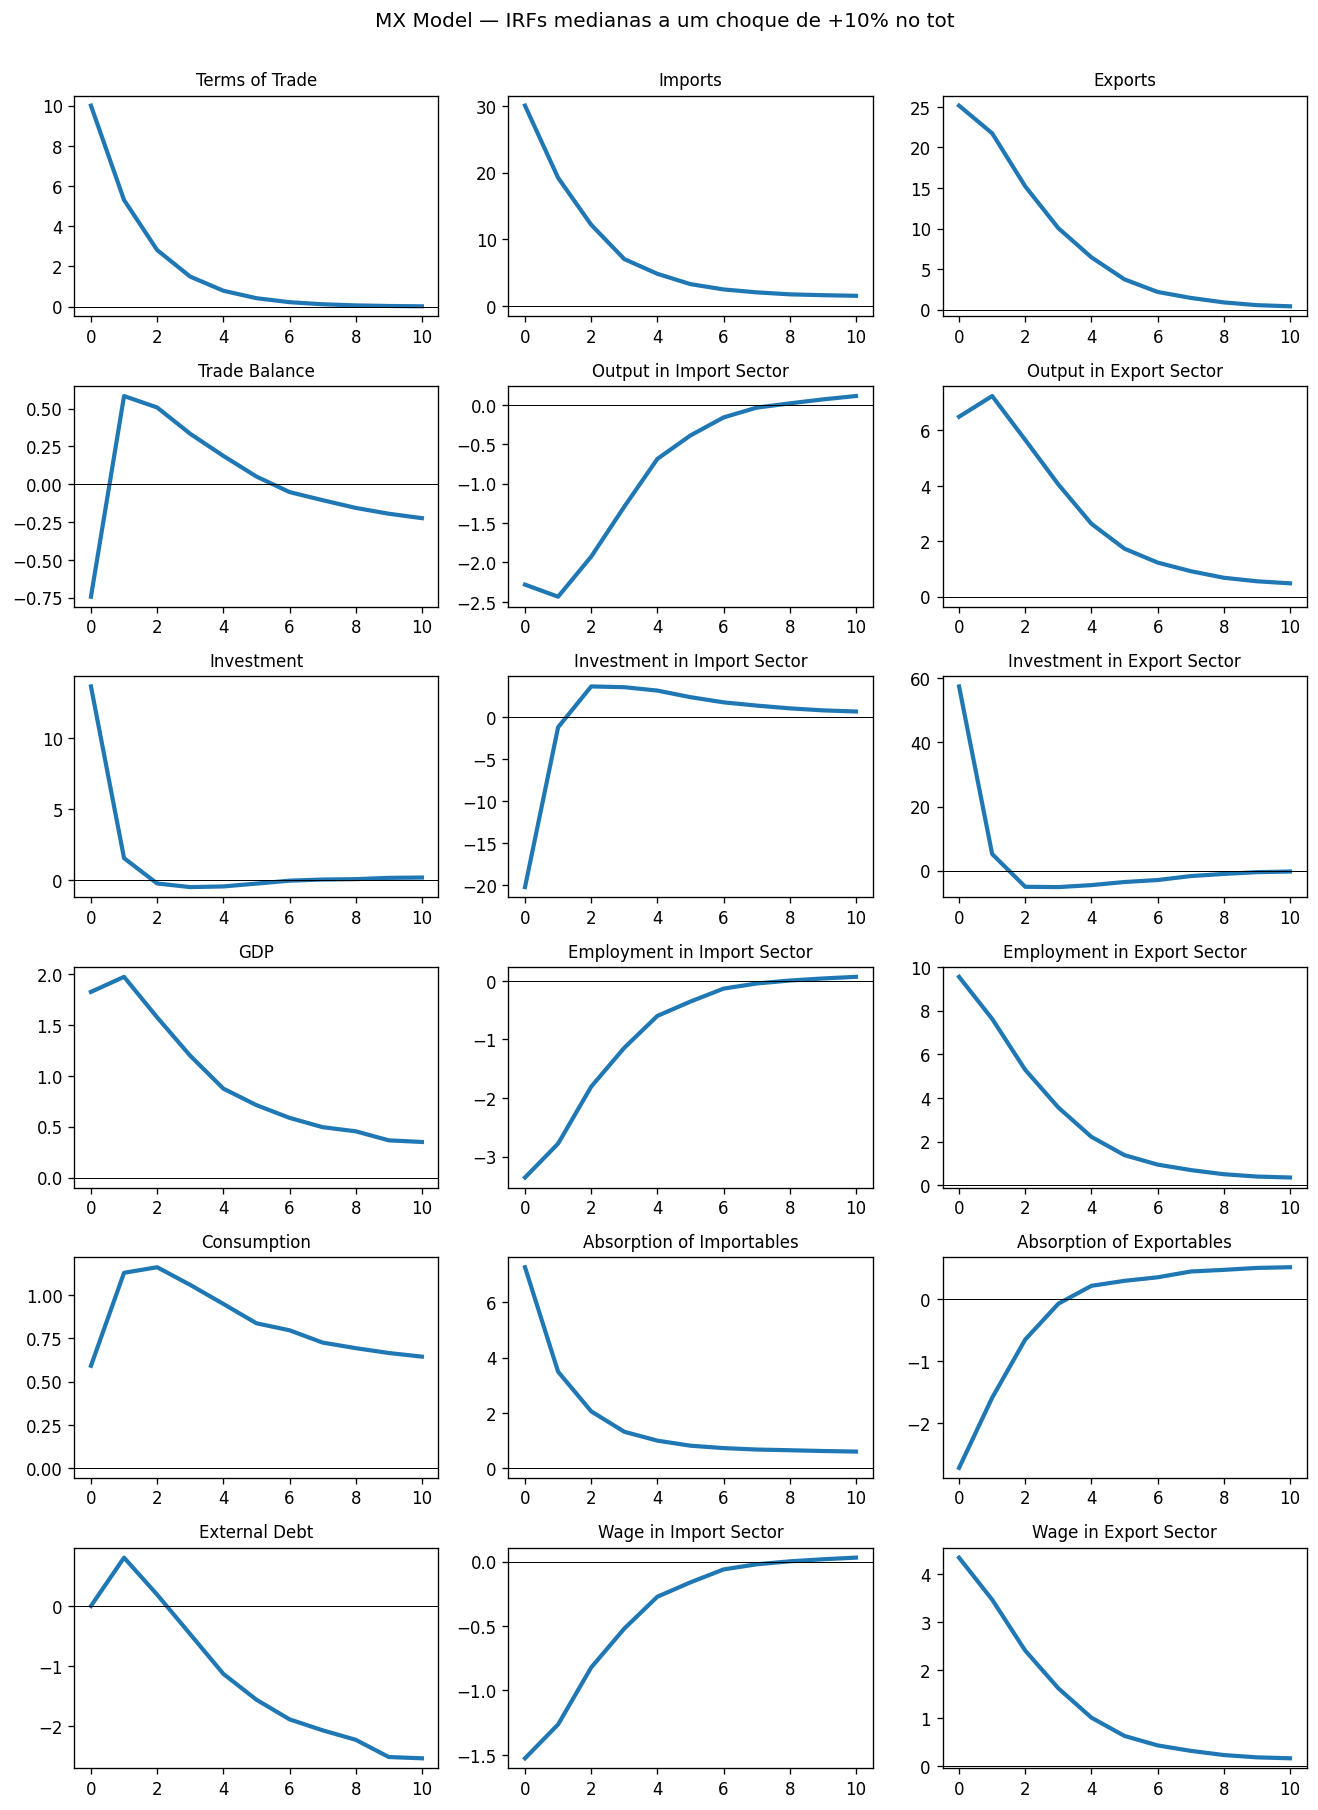
\includegraphics[height=6.2cm]{fig_mx_ir}\\[2pt]
{\tiny MX model, cross-country median IRFs to a $+10\%$ ToT shock (replication).}
\end{column}
\end{columns}
\end{frame}

% ------------------------------------------------------------
% 8b. VARIANCE SHARES: MX vs SVAR  (Tabela 7.6 + resultado)
% ------------------------------------------------------------
\begin{frame}{Variance Explained by ToT Shocks: MX vs.\ SVAR}
\small
Cross-country median of the fraction of each variable's variance explained by
terms-of-trade shocks (Table 7.6):
\vspace{0.3cm}
\begin{center}
\begin{tabular}{lcc}
\toprule
\textbf{Variance share (\%)} & \textbf{MX Model} & \textbf{Empirical SVAR} \\
\midrule
Terms of Trade & 100.0 & 100.0 \\
Trade Balance & 26.9 & 12.2 \\
Output        & 18.0 &  9.8 \\
Consumption   & 24.1 & 10.6 \\
Investment    & 20.3 & 10.2 \\
\bottomrule
\end{tabular}
\end{center}
\vspace{0.4cm}
\begin{block}{Main Result}
\centering
The MX model attributes roughly \textbf{twice as much}
business-cycle variation to ToT shocks as the empirical SVAR.
\end{block}
\end{frame}

% ------------------------------------------------------------
% 9. COUNTRY-LEVEL DETAIL  (Tabela 7.7 por país)
% ------------------------------------------------------------
\begin{frame}{Country-Level Variance Shares (Table 7.7)}
\scriptsize
Fraction of each variable's variance explained by ToT shocks (\%), country by
country: MX model vs.\ empirical SVAR. Ratios can exceed 100 when the model
predicts more ToT-driven variance than the data display.
\vspace{0.15cm}
\begin{center}
\begin{tabular}{lcccccccc}
\toprule
& \multicolumn{2}{c}{Trade Bal.} & \multicolumn{2}{c}{Output}
& \multicolumn{2}{c}{Consump.} & \multicolumn{2}{c}{Invest.}\\
\cmidrule(lr){2-3}\cmidrule(lr){4-5}\cmidrule(lr){6-7}\cmidrule(lr){8-9}
Country & MX & SVAR & MX & SVAR & MX & SVAR & MX & SVAR\\
\midrule
Argentina    &   4.1 & 25.3 &  5.0 & 30.5 &  5.4 & 17.0 &  5.0 & 25.9\\
Bolivia      &  12.5 &  2.5 & 17.9 &  3.5 & 59.6 & 10.6 & 45.1 &  7.6\\
Botswana     &   9.7 & 27.7 & 16.8 & 48.6 &  6.0 & 36.8 & 11.1 & 39.0\\
Brazil       &  60.4 & 43.4 & 15.2 & 10.9 & 14.4 &  3.7 & 19.6 & 16.2\\
El Salvador  &  20.0 & 10.7 & 19.9 & 10.3 & 22.3 & 10.2 & 23.6 & 10.7\\
Guatemala    &  39.1 &  5.4 & 18.1 &  2.5 & 12.1 &  3.4 & 30.4 &  4.8\\
Uruguay      &   4.1 & 17.3 &  8.3 & 34.3 &  6.2 & 32.9 &  3.8 & 14.4\\
Venezuela    &  26.9 & 41.9 & 15.1 & 23.8 &  9.5 & 33.6 &  8.3 & 11.0\\
Zimbabwe     &   3.2 &  7.0 &  4.7 & 10.3 &  7.2 & 33.8 &  2.2 & 16.9\\
\midrule
\textbf{Median (all 51)} & \textbf{26.9} & \textbf{12.2} & \textbf{18.0}
& \textbf{9.8} & \textbf{24.1} & \textbf{10.6} & \textbf{20.3} & \textbf{10.2}\\
\bottomrule
\end{tabular}
\end{center}
\vspace{0.1cm}
\begin{block}{Reading the Table}
\centering
Considerable heterogeneity across countries; the median (Table 7.6) is the
robust summary. Full 51-country table in \texttt{table\_7\_7\_bycountry.csv}.
\end{block}
\end{frame}

\end{document}
